\section{Virtual Memory Management}

Bei der virtuellen Speicherverwaltung erfolgt die Umwandlung von vom ARM Prozessor generierten, virtuellen Adressen in physikalische Adressen durch die \emph{Memory Management Unit} (MMU). Dieses Kapitel enthält die Beschreibung des Designs und der Implementierung der virtuellen Speicherverwaltung des Betriebssystems sowie der Einstellungen der MMU.\\

\subsection{Aufteilung des virtuellen Speichers und Mapping}

Die \emph{VSMAv7} definiert zwei unabhängige Formate für translation tables \cite[S. B3-1318]{ARM:ARM}:

\begin{itemize}
	\item \emph{Short-descriptor format}:
	\begin{itemize}
		\item zweistufige Seitentabelle 
		\item 32-bit Deskriptoren (PTE)
		\item 32-bit virtuelle Eingangsadresse 
		\item bis zu 40-bit große physikalische Ausgangsaddresse
	\end{itemize}
	\item \emph{Long-descriptor format}:
	\begin{itemize}
		\item dreistufige Seitentabelle
		\item 64-bit Deskriptoren (PTE)
		\item verwendet \emph{Large Physical Address Extension} (LPAE)
		\item bis zu 40-bit große virtuelle Eingangsadresse 
		\item bis zu 40-bit große physikalische Ausgangsaddresse
	\end{itemize}
\end{itemize}

Um die Anforderungen an das Betriebssystem zu erfüllen, reicht das zweistufige Seitentabellensystem vollkommen aus. Tabelle \ref{table:GeneralVirtualMemory} fasst die wichtigsten gegebenen Eigenschaften unter Verwendung des Short-descriptor format zusammen.\\

\begin{table}[H]
\begin{tabular}{p{7cm} | p{7cm}}
  \textbf{Eigenschaft} & \textbf{Beschreibung} \\ \hline
  Virtueller Speicher & 4 GB\\  
  Größe eines Page Table Entry (PTE) & 4 Byte \\
  Einträge L1 Page Table & 4096\\
  Einträge L2 Page Table & 256\\
  Speicherbedarf L1 Page Table & 4 Byte * 4096 = 16kB \\
  Speicherbedarf L2 Page Table & 4 Byte * 256 = 1kB\\
  Unterstützte Pagegrößen: & \emph{small page} (4 kB), \emph{large page} (64 kB)\\
  Unterstützte Sectiongrößen: & \emph{section} (1 MB), \emph{supersection} (16 MB)\\
 \end{tabular}
 \caption{Eigenschaften der virtuellen Speicherverwaltung der ARMv7-Architektur}
 \label{table:GeneralVirtualMemory}
\end{table}

\subsection*{Seitentabellen}

Der verwendete ARM Prozessor verfügt über zwei Register (\emph{Translation Table Base Register}, \emph{TTBR0} und \emph{TTBR1}), welche Startadressen von Seitentabellen enthalten können \cite[S. B3-1320]{ARM:ARM}. Diese Register übernehmen die folgende Funktion:

\begin{itemize}
	\item TTBR0: Wird für prozessspezifische Adressen verwendet. Jeder Prozess enthält eine eigene L1-Seitentabelle. Bei einem Kontextwechsel erhält das TTBR0 eine Referenz auf L1-Seitentabelle des neuen Kontextes/Prozesses.
	\item TTBR1: Wird für das Betriebssystem selbst und für memory-mapped I/O verwendet. Diese ändern sich bei einem Kontextwechsel nicht.
\end{itemize}


Abbildung \ref{fig:MemoryMap} zeigt die Speicherverwaltung des Betriebssystems. Die rechte Seite stellt das physikalische Speichermapping dar und wurde dem Datenblatt des ARM \cite[S. 155]{ARM:TRM} entnommen. Die linke Seite zeigt die Aufteilung des virtuellen Speichers.\\

\begin{figure}[H]
	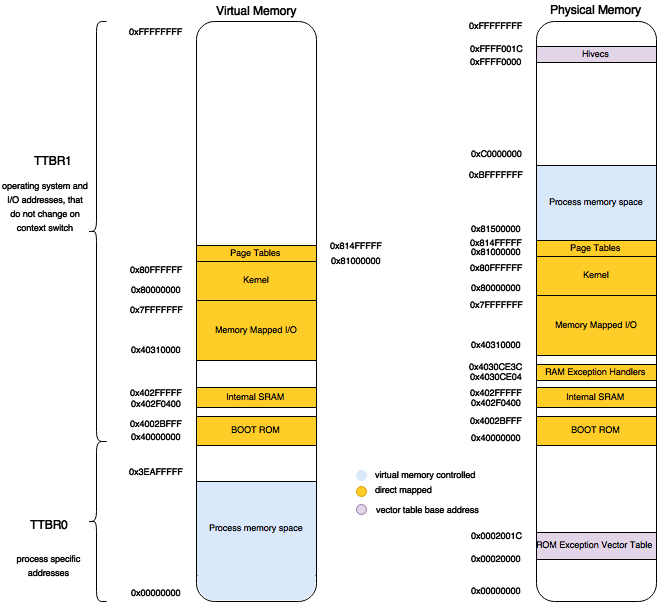
\includegraphics[scale=0.7]{figures/MemoryMap}
	\caption{Memory Map des Betriebssystems}
	\label{fig:MemoryMap}
\end{figure}

\begin{table}[H]
\begin{tabular}{p{7cm} | p{7cm}}
  \textbf{Eigenschaft} & \textbf{Beschreibung} \\ \hline
  Größe der Pages & 4 kB\\
  Speicherbedarf Kernel & 16 MB\\
  Virtueller Speicher für Prozesse & 1003 MB\\
  Physikalischer Speicher für Page Tables	& 5 MB\\
  Max. Anzahl von L1 und L2 Page Tables & 320 L1 Page Tables oder 1 L1 Page Table + 1276 L2 Page  Table\\
  Theoretisch Max. Anzahl von Prozessen & 320\\
 \end{tabular}
 \caption{Eigenschaften der virtuellen Speicherverwaltung des OS}
 \label{table:SpecifiedVirtualMemory}
\end{table}


\lstinputlisting[language=C]{codefiles/region.c}

\subsection{Umwandlung virtueller Adressen zu physikalische Adressen}

Abbildung \ref{fig:largePageTranslation} zeigt die Umwandlung einer vom ARM Prozessor erzeugten virtuellen Adresse in eine physikalische Speicheradresse. Die Umwandlung wird vollständig durch die Prozessor-Hardware durchgeführt.

\begin{figure}[H]
	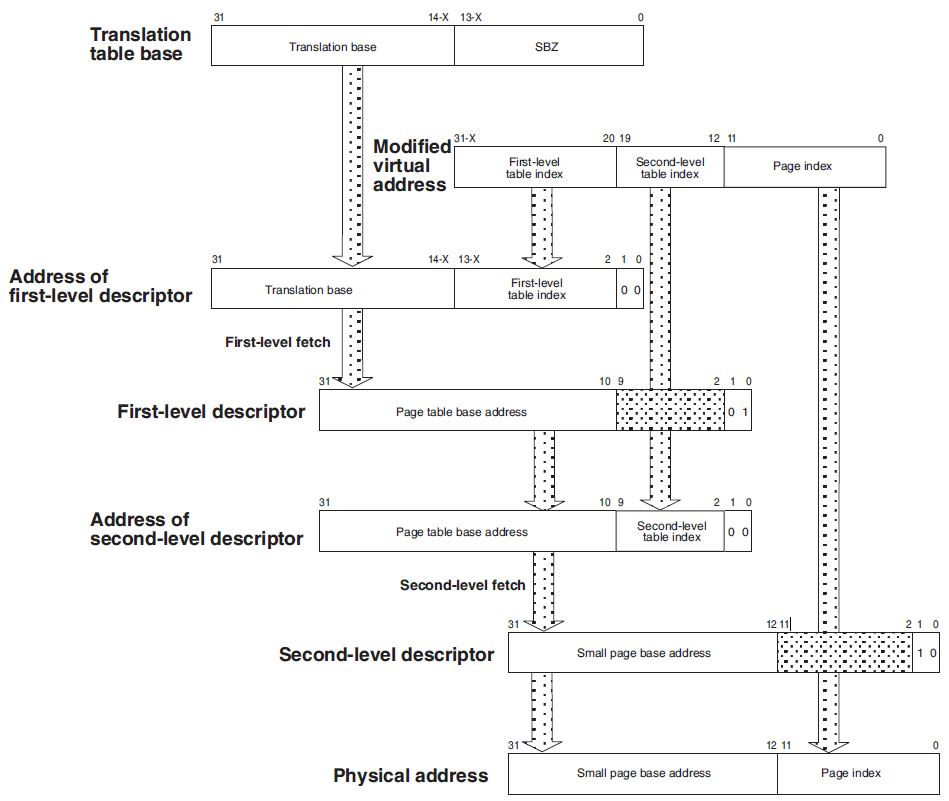
\includegraphics[scale=0.8]{figures/largePageTranslation}
	\caption{Umwandlung einer virtuellen Adresse durch die ARM CPU \cite[S. B3-1337]{ARM:ARM}}
	\label{fig:largePageTranslation}
\end{figure}



\subsection{Allokierung der Page Frames}

Für die Verwaltung der page frames wurde eine Bitsmap verwendet. Abbildung \ref{fig:BitsMap} zeigt das Prinzip.
Die Bitsmap wird durch ein Array der Länge N/8 Bytes realisiert. N steht hier für die Anzahl der page frames. Das i-te Bit im n-ten Byte der Bitsmap definiert den Verwendungsstatus des (n*8 + i) –ten page frame.


\begin{figure}[H]
	\centering
	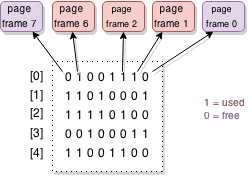
\includegraphics[scale=1]{figures/BitsMap}
	\caption{Beispiel einer Bitsmap zur Verwaltung der Page Frames}
	\label{fig:BitsMap}
\end{figure}



\pagebreak 